\documentclass{beamer}

\usepackage[utf8]{inputenc}
\usepackage[ngerman]{babel}

\usepackage{array}
\usepackage{calc}
\usepackage{graphicx}
\usepackage{amssymb}
\usepackage{amsthm}
\usepackage{mathtools}
% \usepackage{xcolor}

\usepackage[vlined, ruled, linesnumbered]{algorithm2e}
\SetEndCharOfAlgoLine{}

\usepackage{textpos}
\usepackage{color}
\usepackage{tikz}
\usetikzlibrary{shapes, arrows, positioning, decorations.pathmorphing}

\setbeamertemplate{bibliography item}[triangle]

\renewcommand{\thealgocf}{}
\renewcommand{\atop}[2]{\genfrac{}{}{0pt}{2}{#1}{#2}}

\setbeamerfont{quote}{shape=\upshape,family=\rmfamily}

\newcommand{\mc}{\mathcal}
\newcommand{\mb}{\mathbf}
\newcommand{\N}{\mathbb{N}}
\newcommand{\Z}{\mathbb{Z}}
\newcommand{\Q}{\mathbb{Q}}
\newcommand{\R}{\mathbb{R}}
\newcommand{\Sy}{\mathcal{S}}
\newcommand{\tb}[1]{{\textcolor{blue}{#1}}}
\newcommand{\tred}[1]{{\textcolor{red}{#1}}}

\theoremstyle{plain}
\newtheorem{thm}{Satz}[section]
\newtheorem{lem}[thm]{Lemma}
\newtheorem{prop}[thm]{Proposition}
\newtheorem{defn}[thm]{Definition}
\newtheorem{expl}[thm]{Beispiel}
\newtheorem{rem}[thm]{Bemerkung}
\newtheorem{cor}[thm]{Korollar}
\newtheorem{notn}[thm]{Notation}

\usetheme{Boadilla}
\setbeamertemplate{navigation symbols}{} %Leave out navigation symbols
 \setbeamertemplate{footline}
        {
      \leavevmode%
      \hbox{%
      \begin{beamercolorbox}[wd=.333333\paperwidth,ht=2.25ex,dp=1ex,center]{author in head/foot}%
        \usebeamerfont{author in head/foot}\insertshortauthor~~(\insertshortinstitute)
      \end{beamercolorbox}%
      \begin{beamercolorbox}[wd=.333333\paperwidth,ht=2.25ex,dp=1ex,center]{title in head/foot}%
        \usebeamerfont{title in head/foot}\insertshorttitle
      \end{beamercolorbox}%
      \begin{beamercolorbox}[wd=.333333\paperwidth,ht=2.25ex,dp=1ex,right]{date in head/foot}%
        \usebeamerfont{date in head/foot}\insertshortdate{}\hspace*{2em}

    %#turning the next line into a comment, erases the frame numbers
        %\insertframenumber{} / \inserttotalframenumber\hspace*{2ex} 

      \end{beamercolorbox}}%
      \vskip0pt%
    }
    
    
\title[Kryptographie]{Einführung in die Kryptographie}
\subtitle{Ein Überblick\\ \vspace{0.5cm} \footnotesize{Basierend auf einem Vortrag von Mohamed Barakat, TU Kaiserslautern}}
\author[Torchiani]{Carolin Torchiani}
\institute[Uni Koblenz]{\vspace{-0.5cm}\begin{center}
 
\includegraphics[width=27mm]{logo_uni-koblenz}
\end{center}
}

\date{Koblenz, 13.\ April 2015}


\begin{document}

\frame{\titlepage}

\addtobeamertemplate{frametitle}{~}{%
\begin{textblock*}{40mm}[0.75, 0.75](\textwidth, 0\textheight)

\includegraphics[width=27mm]{logo_uni-koblenz}
\end{textblock*}}

\tikzset{pblock/.style = {draw, rectangle split, rectangle split vertical,
                      rectangle split parts=2, very thick, fill=blue!20, rounded corners}}

\begin{frame}{Kryptographie}{~}
\only<1>{\begin{center}
\begin{tikzpicture}
 \node[draw, rectangle, fill=blue!20, rounded corners] (c1) at (-3, 0) {Alice};
 \node[draw, rectangle, fill=blue!20, rounded corners] (c2) at (3, 0) {Bob};
 \draw[-triangle 45] (c1) -- node [above] {Botschaft} (c2);
\end{tikzpicture}
\end{center}
}
\only<2>{
\begin{center}
\begin{tikzpicture}
 \node[draw, rectangle, fill=blue!20, rounded corners] (c1) at (-3, 0) {Alice};
 \node[draw, rectangle, fill=blue!20, rounded corners] (c2) at (3, 0) {Bob};
 \node[draw, rectangle, fill=red!20, rounded corners] (ch) at (0, -2) {Eve};
 \draw[-triangle 45] (c1) -- node [above] {Botschaft} (c2);
 \draw[-triangle 45, decorate, decoration=zigzag] (0, 0) -- (ch);
\end{tikzpicture}
\end{center}
}
\only<3>{
\begin{center}
\begin{tikzpicture}
 \node[pblock] (c1) at (-4, 0) {\nodepart{one} Alice \nodepart{two} Verschlüsselung};
 \node[pblock] (c2) at (4, 0) {\nodepart{one} Bob \nodepart{two} Entschlüsselung};
 \node[draw, rectangle, fill=red!20, rounded corners] (ch) at (0, -2) {Eve};
 \draw[-triangle 45] (c1) -- node [above] {verschlüsselte Botschaft} (c2);
 \draw[-triangle 45, decorate, decoration=zigzag] (0, 0) -- (ch);
\end{tikzpicture}
\end{center}
}
\end{frame}

\begin{frame}{Kryptologie}{~}
 Die moderne \tb{Kryptologie} besteht aus zwei Teilgebieten:
 \begin{itemize}
  \item \tb{Kryptographie:} Entwicklung von Kryptosystemen \\
   $\rightsquigarrow$ Verfahren zur Verschlüsselung (Chiffrieren) von Information
  \item \tb{Kryptoanalyse:} Analyse von Kryptosystemen \\
   $\rightsquigarrow$ Sicherheitsanalyse und Angriffsstragegien
 \end{itemize}
\vspace{0.5cm}
 Griechisch: kryptós = verborgen, gráphein = schreiben \\
 Arabisch: sifr = Null
\end{frame}


\begin{frame}{Ziele der Verschlüsselung}{~}
\begin{itemize}
 \item<1-> \tb{Schutz gegen Abhören:} Geheimcode gegen Lauscher
 \item<2-> \tb{Schutz gegen Veränderung:} Integrität
 \item<3-> \tb{Beweis der Urheberschaft:} Digitale Signaturen
\end{itemize}
\vspace{1cm}
\only<1>{
Die versandte Nachricht soll geheim bleiben, der klassische Einsatzbereich von Verschlüsselungsverfahren. \\
Früher für Militär und Diplomatie, heute für Jedermann.
\begin{itemize}
 \item Telefonieren mit dem Handy
 \item Datenübertragung im Internet
 \item Pay-TV
 \item ...
\end{itemize}
}

\only<2>{
Wer möchte schon, dass die versandte Nachricht von Unbefugten abgeändert wird.
\begin{itemize}
 \item Homebanking
 \item Email
 \item ...
\end{itemize}
}

\only<3>{
Oft ist es wichtig zu wissen, ob derjenige, der eine Nachricht verschickt, sich ausweisen kann bzw. ob eine Nachricht tatsächlich vom Unterzeichner stammt.
\begin{itemize}
 \item Online-Shopping: Abfrage von Kreditkartendaten
 \item Email
 \item ...
\end{itemize}
}
\end{frame}


\begin{frame}{Kodierungstheorie}{~}
\begin{center}
\only<1>{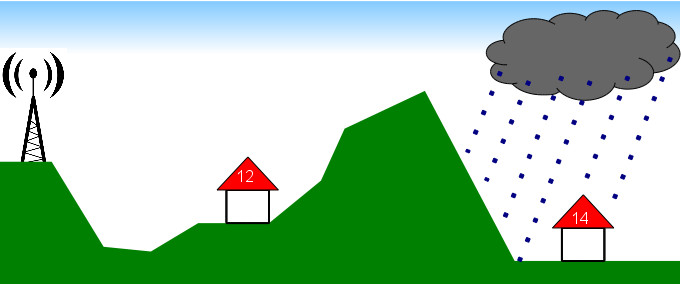
\includegraphics[height=3cm]{bild}}
\only<2>{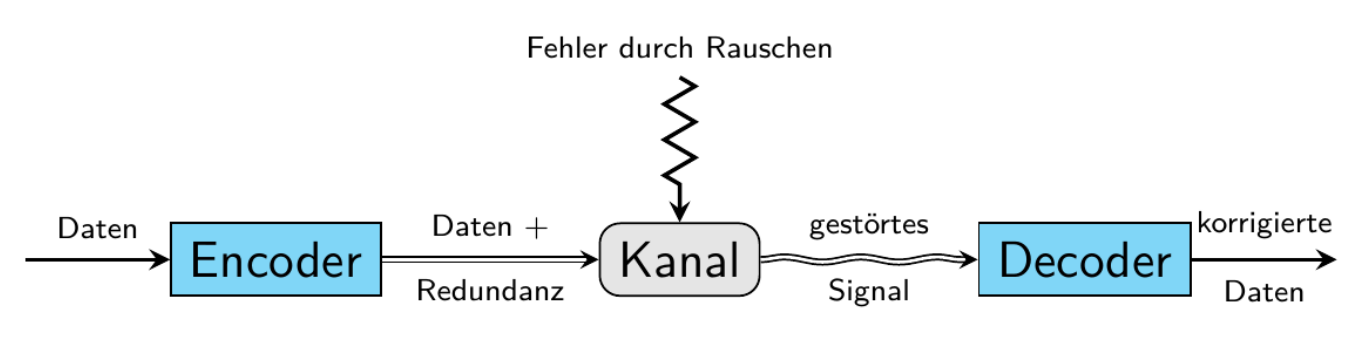
\includegraphics[height=3cm]{kanal_ohne_comic}}
\end{center}
\end{frame}

\begin{frame}{\glqq Definitionen''}{~}
 \begin{block}{}
 Sei $\mc B$ die (endliche) Menge aller \tb{\glqq Buchstaben''} (Alphabet, Ziffern, Bits, Bytes...) und 
 $$\mc N \subset \mc B^{\N}$$
 die Menge aller endlichen Sequenzen (=Tupel) von Buchstaben, d.h. aller \glqq Wörter'', die man aus den Buchstaben bilden kann. Wir nennen $\mc N$ die Menge der \tb{\glqq Nachrichten''}.
 \end{block}
 \pause
 \begin{block}{}
  Ein \tb{Verschlüsselungsalgorithmus} ist eine bijektive Abbildung
  $$\chi: \mc N \rightarrow \mc N.$$
  Die inverse Abbildung $\chi^{-1}: \mc N \rightarrow \mc N$ heißt \tb{Entschlüsselungsalgorithmus}.
 \end{block}
\end{frame}

\begin{frame}{Beispiel}{~}
\tb{Ziffern als Buchstaben:} 
\[\mc B = \{0, 1, 2, 3, 4, 5, 6, 7, 8, 9\} = \Z_{10}\]
\tb{natürliche Zahlen als Nachrichten:}
\[\mc N = \mc B^{\N}, \;\;\; \text{z.\,B. } 236202 \in \mc N\] \pause
\tb{Verschlüsselungsalgorithmus $\chi$:}
\begin{center}addiere auf jeden Buchstaben $6$ modulo $10$, z.\,B. $\chi(236202) = 892868$\end{center} \pause
\tb{Entschlüsselungsalgorithmus $\chi^{-1}$:} \pause
\begin{center}addiere auf jeden Buchstaben $4$ modulo $10$, z.\,B. $\chi^{-1}(892868) = 236202$ \end{center}
\end{frame}


\begin{frame}{SKC}{Definition}
\begin{block}{Symmetrisches Kryptosystem = \underline{S}ecret \underline{K}ey \underline{C}ryptosystem (SKC)}
 Ein \tb{symmetrisches Kryptosystem} mit \tb{Schlüsselraum} $\mc K$ ist eine Familie von Verschlüsselungsalgorithmen $(\chi_k)_{k \in \mc K}$, so dass für jedes $k \in \mc K$ ein eindeutiges $k^{-1} \in \mc K$ existiert mit $$\chi_k^{-1} = \chi_{k^{-1}}.$$ \pause
 Die Elemente von $\mc K$ nennt man \tb{Schlüssel} (=keys). Weiterhin wird verlangt, dass man $k^{-1}$ aus $k \in \mc K$ \glqq leicht'' berechnen kann. Gilt $k^{-1} = k$ für alle $k \in \mc K$, so nennt man das Kryptosystem \tb{involutorisch}. 
\end{block} 
\end{frame}

\begin{frame}{SKC}{~}
 \begin{block}{Beispiel für ein SKC}
  \begin{itemize}[<+->]
   \item Die Menge der Buchstaben \tb{$\mc B$} ist gegeben duch die Elemente $\{0, \dots, 9\} = \Z_{10}$. 
   \item Die Nachrichtenmenge \tb{$\mc N$} besteht aus allen endliche Ziffernfolgen, enthält z.B. $3$, $17$, $1456$, $14923040$.
   \item Die Schlüsselmenge \tb{$\mc K$} ist ebenfalls gegeben durch $\Z_{10}$. 
   \item Ein Element $\chi_k: \mc N \rightarrow \mc N$ der Familie von Verschlüsselungsalgorithmen \tb{$(\chi_k)_{k \in \mc K}$} hat die Vorschrift $$(b_1, \dots, b_n) \mapsto (b_1 + k, \dots, b_n + k).$$ 
   Beispiel mit $k = 3 \in \Z_{10}$: $\chi_3(13679) = 46902$
   \item Der zu $\chi_k$ gehörige Entschlüsselungsalgorithmus ist \tb{$\chi_k^{-1} = \chi_{-k}$}.\\
   Beispiel: Der Entschlüsselungsalgorithmus von $\chi_3$ ist $\chi_{-3} = \chi_{7}$. 
  \end{itemize}
 \end{block}
\end{frame}

\begin{frame}{Strom-Chiffren}{~}
 \begin{block}{Erinnerung}
  Eine \tb{Permuation} auf einer endlicher Menge $\mc B$ ist eine bijektive Abbildung $\sigma: \mc B \rightarrow \mc B$. Die Menge aller Permutationen auf $\mc B$ wird mit $\Sy_{\mc B}$ bezeichnet.
 \end{block}
\pause
 \begin{block}{Strom-Chiffre}
 Eine \tb{Strom-Chiffre} ist ein symmetrisches Kryptosystem $(\chi_k)_{k \in \mc K}$ mit folgenden Eigenschaften:
 \begin{enumerate}
  \item Jeder Schlüssel $k \in \mc K$ ist ein Tupel von Permutationen $(\sigma_i)_{i=1}^{l_k}$ auf der Buchstabenmenge $\mc B$, d.h. $\sigma_i \in \Sy_{\mc B}$ für alle $i = 1, \dots, l_k$. \\ \pause
  Die Zahl $l_k \in \N$ heißt \tb{Schlüssellänge} von $k$. \\
    \pause
  \item Für eine Nachricht $n = (n_j)_{j=1}^h \in \mc N \subset \mc B^{\N}$ gilt 
   $$(\chi_k(n))_j = \sigma_{(j \mod l_k)}(n_j)$$
   für alle $k \in \mc K$ und $j = 1, \dots, n$.
 \end{enumerate}
 \end{block}
\end{frame}

\begin{frame}{Caesar-Chiffre}{Beispiel einer Strom-Chiffre}
 \begin{columns}[T]
  \begin{column}{.7\textwidth}
 Die \tb{Caesar-Chiffre} ist wie folgt aufgebaut: 
 \begin{itemize}
  \item $\mc B = \{A, B, C, \dots, Z\}$
  \item $\mc K = \{1, \dots, 25\}$
  \item Schlüssellänge $l_k = 1$ für alle $k \in \mc K$ \pause
  \item Die Permuation $\sigma_k$ verschiebt das Alphabet um $k$ Stellen, d.h. falls $k = 3$:
  \begin{center}
 \texttt{\tred{A}BCDEFGH\tred{I}KJLMNOPQRS\tred{T}UVWXYZ}\\
 \texttt{\tred{X}YZABCDE\tred{F}GHIJKLMNOP\tred{Q}RSTUVW}
 \end{center}
 Aus
 \begin{center} 
\texttt{ALEA IACTA EST}  
 \end{center}
 wird 
 \begin{center}
\texttt{XIBX FXZQX BPQ.}  
 \end{center} 
 \end{itemize}
 \end{column}
 
 \begin{column}{0.3\textwidth}
  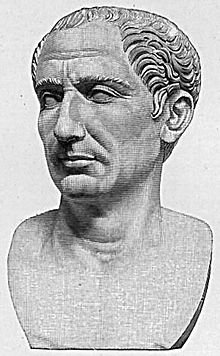
\includegraphics[width=\textwidth]{caesar}
 \end{column}
 \end{columns}
\end{frame}

\begin{frame}{Caesar-Chiffre}{Beispiel einer Strom-Chiffre}
Mithilfe zweier gegeneinander verdrehbarer Scheiben kann man eine Ver- und Entschlüsselungsmaschine bauen. 

\vspace{0.5cm}
\begin{center}
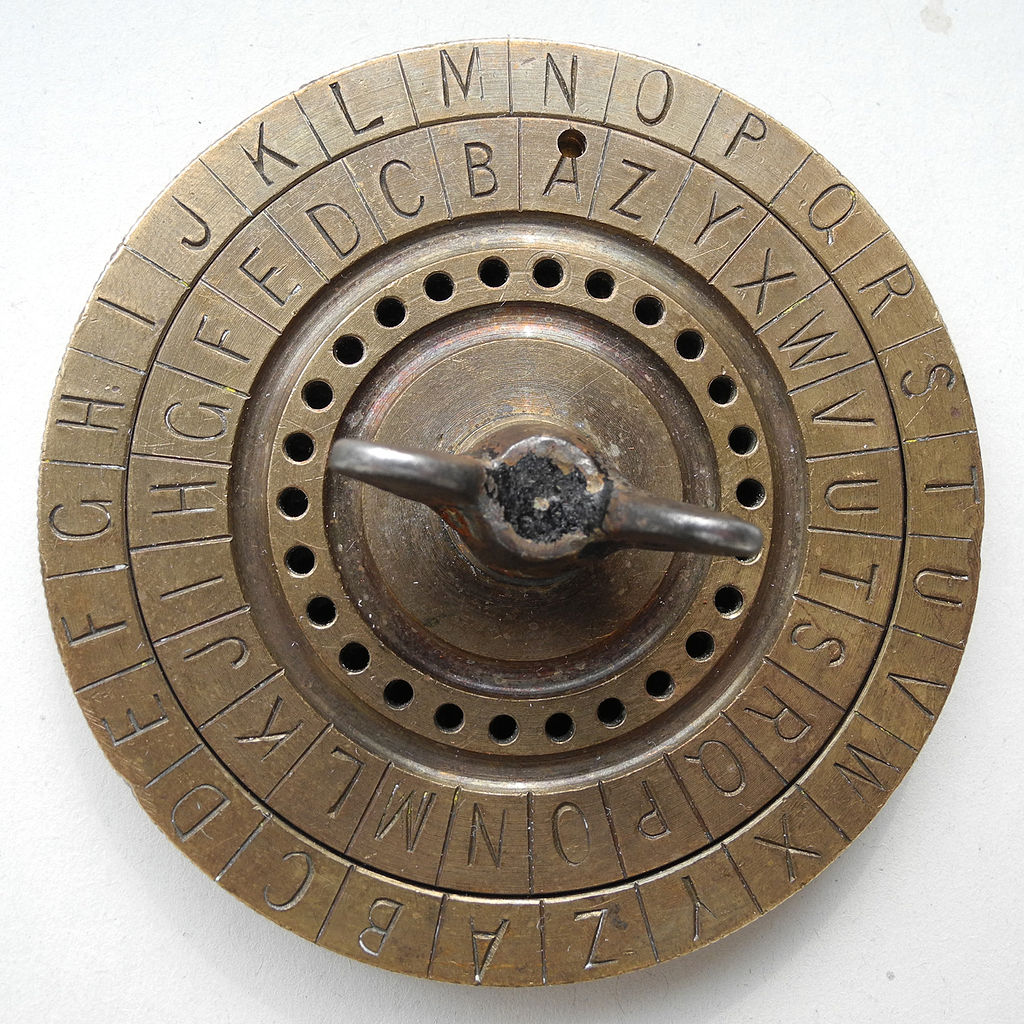
\includegraphics[height=0.5\textheight]{caesar-chiffre}
\end{center}
\end{frame}

\begin{frame}{Caesar-Chiffre}{~}

\begin{itemize}
 \item Die Caesar-Chiffre ist eine sogenannte \tb{monoalphabetische Verschlüsselung}: Jedem Buchstaben im Klartext entspricht genau ein Buchstabe im verschlüsselten Text (=Chiffretext). 
%  Das Alphabet wird \glqq verwürfelt''.
 \item \textbf{Knacken der Caesar-Chiffre}: \pause Ausprobieren der 25 verschiedenen Möglichkeiten
\end{itemize}

\end{frame}

\begin{frame}{Monoalphabetische Verschlüsselung}{Anzahl der Schlüssel}
  Statt nur zu verschieben, kann man bei einer monoalphabetischen Verschlüsselung \textbf{jegliche Permutation} des Alphabets $$\sigma: \{\texttt{A, \dots, Z}\} \rightarrow \{\texttt{A, \dots, Z}\}$$
 als Verschlüsselungsalgorithmus nutzen, um das Alphabet zu \glqq verwürfeln''. \\
 Insgesamt gibt es dafür
 $$26! = 403 291 461 126 605 635 584 000 000 \sim 2^{88}$$
 Möglichkeiten. 
 \begin{center}
 \textbf{Knacken durch Ausprobieren ist nicht mehr möglich!}  
 \end{center}
\end{frame}

\begin{frame}{Monoalphabetische Verschlüsselung}{Angriffsstragegie}
 Eine monoalphabetische Verschlüsselung kann durch eine \tb{Häufigkeitsanalyse} genknackt werden.\\
 (E ist der häufigste Buchstabe, Q tritt nur im Paar QU auf.) 
 \vspace{0.5cm}
 \begin{center}
 \footnotesize{
 \begin{tabular}{|l r|l r|l r|l r|l r|l r|}
  \hline
  \multicolumn{12}{|c|}{Häufigkeitsverteilung der Einzelbuchstaben in deutscher Sprache}\\
  \hline
  \hline
  A & 6.51 & F & 1.66 & K & 1.21 & P & 0.79 & U & 4.35 & Z & 1.13 \\
  B & 1.89 & G & 3.01 & L & 3.44 & Q & 0.02 & V & 0.67 & & \\
  C & 3.06 & H & 4.76 & M & 2.53 & R & 7.00 & W & 1.89 & & \\
  D & 5.08 & I & 7.55 & N & 9.78 & S & 7.27 & X & 0.03 & & \\
  E & 17.40& J & 0.27 & O & 2.51 & T & 6.15 & Y & 0.04 & & \\
  \hline
 \end{tabular}
 
 \vspace{0.5cm}
 \begin{tabular}{|c|c|c|c|c|c|c|c|c|c|}
 \hline
 \multicolumn{10}{|c|}{Häufigkeitsverteilung von Buchstabenpaaren in deutscher Sprache}\\
  \hline 
  \hline
  EN & ER & CH & TE & DE & ND & EI & IE & IN & ES \\
  \hline
  3.88 & 3.75 & 2.75 & 2.26 & 2.0 & 1.99 & 1.88 & 1.79 & 1.67 & 1.52 \\
  \hline
 \end{tabular}
 }
 \end{center}
 
\end{frame}

\begin{frame}{Vigenère-Verschlüsselung}{~}
 Ziel: \textbf{Veschleierung der Häufigkeitsverteilung} \pause
 
 \begin{block}{Vigenère-Verschlüsselung}{~}
  \begin{itemize}
   \item Benannt nach Blaise de Vigenère (1523-1596).
   \item Benutzt verschiedene monoalphabetische Verschlüsselungen im Wechsel (\tb{polyalphabetische Verschlüsselung}).
   \item Bestimmung des jeweils aktuellen Alphabets erfolgt aus dem sogenannten \tb{Vigenère-Quadrat} mithilfe eines \tb{Schlüsselworts}. 
  \end{itemize}

 \end{block}
\end{frame}

\begin{frame}{Vigenère-Verschlüsselung}{Vigenère-Quadrat}
 \begin{center}
  \setlength{\tabcolsep}{1mm}
 \small{
 \texttt{
  \begin{tabular}{|cccccccccccccccccccccccccc|}
  \hline 
  A & B & C & D & E & F & G & H & I & J & K & L & M & N & O & P & Q & R & S & T & U & V & W & X & Y & Z \\
  \hline
  \hline
  A & B & C & D & E & F & G & H & I & J & K & L & M & N & O & P & Q & R & S & T & U & V & W & X & Y & Z \\
  B & C & D & E & F & G & H & I & J & K & L & M & N & O & P & Q & R & S & T & U & V & W & X & Y & Z & A \\
  C & D & E & F & G & H & I & J & K & L & M & N & O & P & Q & R & S & T & U & V & W & X & Y & Z & A & B \\
  D & E & F & G & H & I & J & K & L & M & N & O & P & Q & R & S & T & U & V & W & X & Y & Z & A & B & C \\
  E & F & G & H & I & J & K & L & M & N & O & P & Q & R & S & T & U & V & W & X & Y & Z & A & B & C & D \\
  F & G & H & I & J & K & L & M & N & O & P & Q & R & S & T & U & V & W & X & Y & Z & A & B & C & D & E \\
  G & H & I & J & K & L & M & N & O & P & Q & R & S & T & U & V & W & X & Y & Z & A & B & C & D & E & F \\
  H & I & J & K & L & M & N & O & P & Q & R & S & T & U & V & W & X & Y & Z & A & B & C & D & E & F & G \\
  I & J & K & L & M & N & O & P & Q & R & S & T & U & V & W & X & Y & Z & A & B & C & D & E & F & G & H \\
  \vdots & \vdots & \vdots & \vdots& \vdots & \vdots & \vdots& \vdots& \vdots& \vdots& \vdots& \vdots& \vdots& \vdots& \vdots& \vdots& \vdots& \vdots& \vdots& \vdots& \vdots& \vdots& \vdots& \vdots& \vdots& \vdots \\
   X & Y & Z & A & B & C & D & E & F & G & H & I & J & K & L & M & N & O & P & Q & R & S & T & U & V & W \\
   Y & Z & A & B & C & D & E & F & G & H & I & J & K & L & M & N & O & P & Q & R & S & T & U & V & W & X \\
   Z & A & B & C & D & E & F & G & H & I & J & K & L & M & N & O & P & Q & R & S & T & U & V & W & X & Y \\
  \hline
  \end{tabular}
 }
 }
 \end{center}
\end{frame}

\begin{frame}{Vigenère-Verschlüsselung}{Beispiel}
 Mit dem Schlüssel \tb{\texttt{BRUTUS}} wird Caesars \tb{\texttt{ALEA IACTA EST}} zu: 
   
   \setlength{\tabcolsep}{1mm}
   \begin{center}
   \small{
   \texttt{
   \begin{tabular}{|c||cccccccccccccccccccccccccc|}
  \hline 
   & A & B & C & D & E & F & G & H & I & J & K & L & M & N & O & P & Q & R & S & T & U & V & W & X & Y & Z \\
  \hline
  \hline
 \tb B & \tred B & C & D & E & F & G & H & I & J & K & L & M & N & O & P & Q & R & S & T & U & V & W & X & Y & Z & A  \\
 \tb R & R & S & T & U & V & W & X & Y & Z & A & B & \tred C & D & E & F & G & H & I & J & K & L & M & N & O & P & Q  \\
 \tb U & U & V & W & X & \tred Y & Z & A & B & C & D & E & F & G & H & I & J & K & L & M & N & O & P & Q & R & S & T \\
 \tb T & \tred T & U & V & W & X & Y & Z & A & B & C & D & E & F & G & H & I & J & K & L & M & N & O & P & Q & R & S \\
 \tb U & U & V & W & X & Y & Z & A & B & \tred C & D & E & F & G & H & I & J & K & L & M & N & O & P & Q & R & S & T  \\
 \tb S & \tred S & T & U & V & W & X & Y & Z & A & B & C & D & E & F & G & H & I & J & K & L & M & N & O & P & Q & R \\
 \tb B & B & C & \tred D & E & F & G & H & I & J & K & L & M & N & O & P & Q & R & S & T & U & V & W & X & Y & Z & A  \\
 \tb R & R & S & T & U & V & W & X & Y & Z & A & B & C & D & E & F & G & H & I & J & \tred K & L & M & N & O & P & Q  \\
 \tb U & \tred U & V & W & X & Y & Z & A & B & C & D & E & F & G & H & I & J & K & L & M & N & O & P & Q & R & S & T \\
 \tb T & T & U & V & W & \tred X & Y & Z & A & B & C & D & E & F & G & H & I & J & K & L & M & N & O & P & Q & R & S \\
 \tb U & U & V & W & X & Y & Z & A & B & C & D & E & F & G & H & I & J & K & L & \tred M & N & O & P & Q & R & S & T  \\
 \tb S & S & T & U & V & W & X & Y & Z & A & B & C & D & E & F & G & H & I & J & K & \tred L & M & N & O & P & Q & R \\
  \hline
  \end{tabular}
  }
  }
  
  \vspace{0.5cm}
  \texttt{\tred{BCYT CSDKU XML}}
  \end{center}
\end{frame}

\begin{frame}{Vigenère-Verschlüsselung}{Beispiel}

 Die Vigenère-Verschlüsselung ist eine Strom-Chiffre: 
 
 \begin{itemize}[<+->]
  \item \textbf{Schlüsselraum $\mc K$:} parametrisiert durch die Menge aller Wörter auf dem Standardalphabet $\mc A = \{\text{\tb{\texttt{A, B, C, \dots}}}\}$  \\ Beispielwort: \tb{\texttt{BRUTUS}}
  \item \textbf{Länge $l_k$ eines Schlüssels $k \in \mc K$:} Länge des Wortes \\ Bsp.: $l_k = 6$
  \item \textbf{Schlüssel $k \in \mc K$:} Tupel von $l_k$ Permutationen $(\sigma_i)_{i=1}^{l_k}$ \\ 
  Bsp.: $\sigma_1$ verschiebt das Alphabet um $1$ ($\hat =$ \tb{\texttt{B}}) Buchstaben.\\
  \hspace{0.9cm}$\sigma_2$ verschiebt das Alphabet um $17$ ($\hat = $ \tb{\texttt{R}}) Buchstaben.\\
  \hspace{5cm}$\vdots$
  \item \textbf{Verschlüsselung einer Nachricht $(n_j)_{j=1}^h \in \mc N$:} $n_j \mapsto \sigma_{(j \mod l_k)}(n_j)$ \\ Bsp. für $j = 8$ mit $j \equiv 2 \mod l_k$: \\
  Der $8$-te Buchstabe \tb{\texttt{T}} von \tb{\texttt{ALEA IACTA EST}} wird durch $\sigma_2$ veschlüsselt und um 17 ($\hat = $ \tb{\texttt{R}}) Buchstaben auf \tb{\texttt{K}} verschoben.
 \end{itemize}
\end{frame}

\begin{frame}{Vigenère-Verschlüsselung}{Historischer Hintergrund}
\begin{itemize}
 \item Die Vigenère-Verschlüsselung ist mit einer naiven Häufigkeitsanalyse nicht zu knacken. Sie galt bis Mitte des 19.\ Jahrhunderts als sicher.
 \item \textbf{Wesentliche Schwäche:} Zyklischer Charakter \pause
 \item Erstmalige Entschlüsselung 1854 durch Charles Babbage
 \item Entschlüsselung durch \textbf{Kasikitest}:
 \begin{itemize}
 \item Ermittelung der Schlüssellänge $l_k$ des Schlüssels $k$
 \item $l_k$ Häufigkeitsanalysen (analog zur Caesar-Chiffre)
\end{itemize}
\end{itemize}
 
\end{frame}

\begin{frame}{Vigenère-Verschlüsselungen}{Angriffsstragegie}

Abgehörte Botschaft:

\begin{quote}
\small{\texttt{
WUB\tred{EFIQ}LZURMVOFEHMYMWTIXCGTMPIFKRZUPMVOIRQMMWOZMPULMBNYVQQQ
MVMVJLEYMHFEFNZ\tb{PSDLPPSDLP}EVQM\textcolor{green}{WCXYM}DAVQE\tred{EFIQ}CAYTQO\textcolor{green}{WCXYM}WMSEM
EFCFWYEYQ\textcolor{cyan}{ETRL}IQYCGMTWCWFBSMYFPLRXTQYEEXMRULUKSGWFPTLRQAERLE
EXMRULUKSGWFPTLRQAERLUVPMVYQYCXTWFQLMTELSFJPQEHMOZCIWCIWFPZ
SLMAEZIQVLQMZVPPXAWCSMZMORVGVVQSZ\textcolor{cyan}{ETRL}QZPBJAZVQIYXEWWOICCGDW
HQMMVOWSGNTJPFPPAYBIYBJUTWRLQKLLLMDPYVACDCFQNZPIFPPKSDVPTID
GXMQQVEBMQALKEZMGCVKUZKIZBZLIUAMMVZ}}
\end{quote}

Wiederholt auftretende Zeichenfolgen:

\begin{center}
 \small{\texttt{\tred{EFIQ} \; \tb{PSDLP} \; \textcolor{green}{WCXYM} \; \textcolor{cyan}{ETRL} }}
\end{center}
\end{frame}

\begin{frame}{Vigenère-Verschlüsselungen}{Angriffsstragegie}
 
 \textbf{Bestimmung der Schlüssellänge \vspace{0.5cm}}
 
 \footnotesize{
 \setlength{\tabcolsep}{1mm}
 \begin{tabular}{|c|c|ccccccccccccccccccc|}
  \hline
  Zeichen- & Zwischen- & \multicolumn{19}{c|}{Teiler der Zwischenraumlänge $\hat = $ mögliche Schlüssellänge} \\
  folge & raum & 2 & 3 & 4 & 5 & 6 & 7 & 8 & 9 & 10 & 11 & 12 & 13 & 14 & 15 & 16 & 17 & 18 & 19 & 20 \\
  \hline
  \tred{EFIQ} & 95 &  &  &  & $\times$ &  &  &  &  &  &  &  &  &  &  &  &  &  & $\times$ &  \\
  \tb{PSDLP} & 5 &  &  & & $\times$ &  &  &  &  &  &  &  &  &  &  &  & & &  &  \\
  \textcolor{green}{WCXYM} & 20 & $\times$ &  & $\times$ & $\times$ &  &  &  &  & $\times$ &  &  &  &  & & &  &  &  & $\times$ \\
  \textcolor{cyan}{ETRL}   & 120 & $\times$ &  & $\times$ & $\times$ & $\times$ &  & $\times$ &  & $\times$ &  & $\times$ &  & & $\times$ &  &  & &  & $\times$ \\
  \hline
 \end{tabular}
 }
 \pause
 \normalsize{
 \vspace{0.5cm}
 \begin{center}
 Wahrscheinliche Schlüssellänge: \; $5$
 \end{center}}
  \vspace{0.5cm}
 
 \pause
 \textbf{Anschließend:} $5$ Häufigkeitsanalysen
 \end{frame}

 \begin{frame}{Block-Chiffren}{~}
 
 \begin{block}{Block-Chiffre}
 Bei einer Blockchiffre wird auf Blöcken von Buchstaben, statt auf einzelnen Buchstaben operiert.
 \end{block}
 
 \vspace{0.5cm}
 
 \begin{itemize}
  \item Spartanische Skytale
  \item DES, $3$DES, AES
 \end{itemize}

 \end{frame}

 \begin{frame}{Die Spartanische Skytale}{Eine Block-Chiffre}
 
 \textbf{Verwendung:} Spartaner (ca.~500 v.~Chr.) \pause
 
 \vspace{0.5cm}
 \textbf{Verschlüsseln:} Wähle einen Stab, wickele einen Papierstreifen mehrfach darum und schreibe dann den Text auf den Streifen, so dass jeder Buchstabe auf einer neuen Papierbahn liegt.
 \begin{center}
  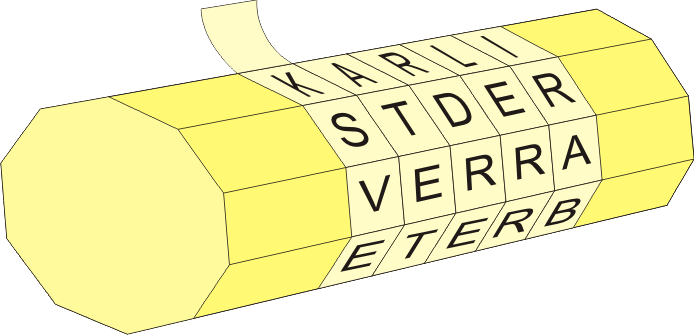
\includegraphics[width=0.4\textwidth]{skytale}
 \end{center}
\vspace{0.5cm} \pause
\textbf{Entschlüsseln:} Aufrollen auf Stab derselben Dicke
 \end{frame}

 \begin{frame}{Moderne Kryptographie}{~}
 \setbeamertemplate{caption}{\raggedright\insertcaption\par}
  \begin{columns}
   \begin{column}{0.3\textwidth}
   \begin{center}
    \begin{figure}
    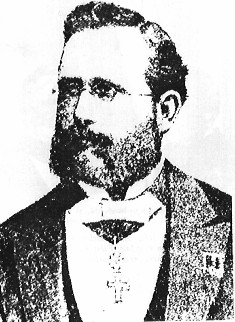
\includegraphics[height=0.3\textheight]{kerkhoffs}
    \caption{Auguste Kerkhoffs 1835--1903}
    \end{figure}
    \end{center}
   \end{column}
   \begin{column}{0.6\textwidth}
  Auguste Kerkhoffs, ein niederländischer Linguist und Kryptograph, formulierte in einer Arbeit von 1883 ein Grundprinzip der modernen Kryptographie:
 \end{column}
  \end{columns} \pause
  \begin{exampleblock}{Kerkhoffs Prinzip}
   Die Sicherheit eines Verschlüsselungsverfahrens darf \underline{nicht} auf der Geheimhaltung des Verschlüsselungsalgorithmus basieren, sondern auf der des Schlüssels.
  \end{exampleblock}
 \end{frame}

 \begin{frame}{One-Time-Pad}{Einmal-Verschlüsselung via Strom-Chiffre}
  \setbeamertemplate{caption}{\raggedright\insertcaption\par}
  \begin{columns}
   \begin{column}{0.6\textwidth}
    \tb{Vernam-Chiffre:} Strom-Chiffre, deren Schlüssellänge mindestens so lang ist wie der zu veschlüsselnde Text \\
    \tb{One-Time-Pad:} Vernam-Chiffre, bei der jeder Schlüssel nur genau einmal benutzt wird
   \end{column}
   \pause
   \begin{column}{0.3\textwidth}
    \begin{center}
    \begin{figure}
     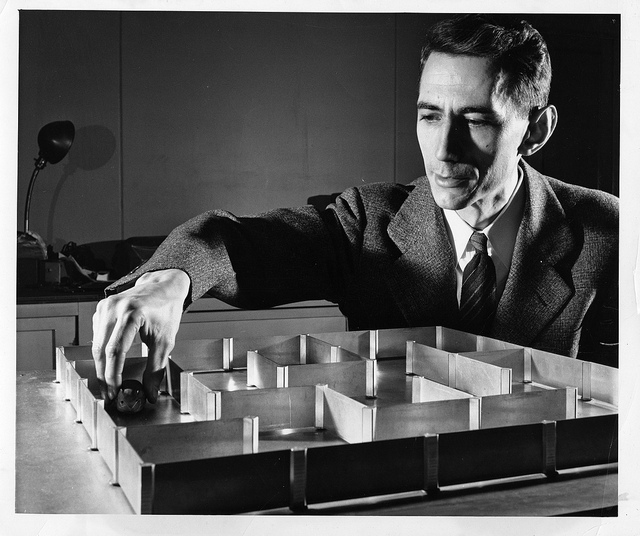
\includegraphics[height=0.3\textheight]{shannon}
     \caption{Claude Shannon 1916--2001}
     \end{figure}
    \end{center}
   \end{column}
  \end{columns}
  
  \begin{exampleblock}{Satz (Shannon, 1948)}
   Das One-Time-Pad bietet perfekte kryptographische Sicherheit.
  \end{exampleblock}
 \end{frame}

 \begin{frame}{Enigma}{Verschlüsselung beim deutschen Militär}
 
  \begin{block}{Enigma -- polyalphabetische Verschlüsselung via Strom-Chiffre }
   \begin{itemize}
    \item Erfinder: Arthur Scherbius (1878--1929)
    \item Anmeldung des Patents: 1918
    \item Nutzung: 1924--1945 durch deutsches Militär und andere Dienste
    \item Prinzip: Rotor-Schlüsselmaschine (auch in anderen Ländern verbreitet)
   \end{itemize}

  \end{block}

 \end{frame}
  \begin{frame}{Enigma}{Verschlüsselung beim deutschen Militär}
    \begin{columns}
    \begin{column}{0.3\textwidth}
  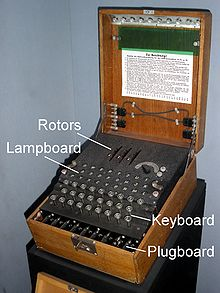
\includegraphics[width=\textwidth]{enigma_maschine}   
    \end{column}
  \begin{column}{0.3\textwidth}
  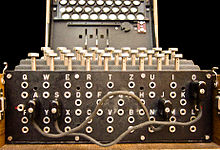
\includegraphics[width=\textwidth]{enigma_stecker}   
    \end{column}
    \begin{column}{0.3\textwidth}
  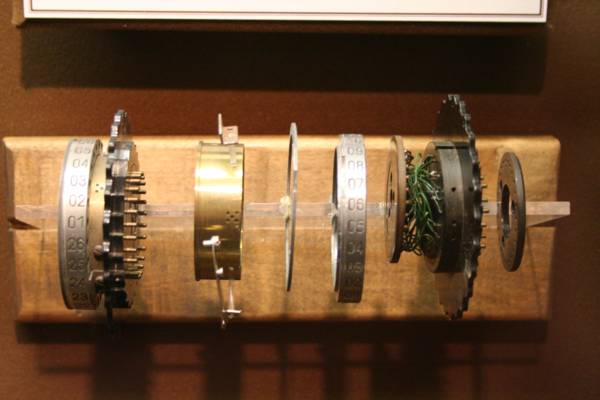
\includegraphics[width=\textwidth]{enigma_walzen}   
    \end{column}
   \end{columns}
 \end{frame}
 
 
 \begin{frame}{Enigma}{Verschlüsselung beim deutschen Militär} 
 
 \begin{block}{Eckdaten der Enigma}
 \begin{itemize}[<+->]
  \item polyalphabetische Stromchiffre
  \item ca.~$2 \cdot 10^{23} \approx 2^{77}  \approx |\mc K|$ Grundeinstellungen\\
  \item Standardalphabet $\mc B = \{A, B, C, \dots, Z\}$
  \item Schlüssellänge $l = 26 \cdot 25 \cdot  26 = 16900$\\
  $\rightsquigarrow$ Kasikitest wertlos bei Nachrichten der Länge $h \leq 16900$ \\
  \hspace{0.3cm} (Vorgabe: Nachrichtenlänge $h < 250$ Zeichen, SMS: $160$ Zeichen)
  \item Schlüssel gegeben durch $(\sigma_i)_{i=1}^{16900} \in \mc K$ \\
  ($\sigma_i$ ist jeweils eine Permutation des Alphabets $\mc B$.)
  \item \textbf{involutorisch} \\
  ($\sigma_i^2(n) = \sigma_i(\sigma_i(n)) = n$ für alle $n \in \mc B$, $i \in [16900]$)
  \item \textbf{fixpunktfrei}\\
  ($\sigma_i(n) \neq n$ für alle $n \in \mc B$, $i \in [16900]$)
 \end{itemize}
 \end{block}
  \end{frame}
  
  
    \begin{frame}{Enigma}{Verschlüsselung beim deutschen Militär} 
  
   \begin{block}{Bedienung}
      \begin{itemize}[<+->]
       \item Einstellung der Walzen, Ringe und Steckerverbindungen gemäß des Tagesschlüssels (in Codebüchern festgehalten)
       \item Sender: 
           \begin{itemize}[<+->]
           \item für jeden Funkspruch zufällige Auswahl einer Grundeinstellung und eines Spruchschlüssels (jeweils drei Buchstaben)
          \item Verschlüsselung des Spruchschlüssels mithilfe der Grundeinstellung
          
	  \item unverschlüsselte Übertragung der Grundeinstellung und Übertragung des verschlüsselten Spruchschlüssels am Anfang der Nachricht
	  \item danach: Übertragung der mit dem Spruchschlüssel veschlüsselten Nachricht
	  \end{itemize}
       \item Empfänger:
        \begin{itemize}[<+->]
        \item Entschlüsselung des Spruchschlüssels mithilfe der Grundeinstellung
        \item Entschlüsselung der Nachricht mithilfe des Spruchschlüssels
        \end{itemize}
      \end{itemize}

   \end{block}

  \end{frame}
  
  
   \begin{frame}{Enigma}{Verschlüsselung beim deutschen Militär} 
    \begin{block}{Skrukturelle Schwächen der Enigma}
     \begin{itemize}
      \item involutorisch
      \item fixpunktfrei
      \item Sicherheit basiert auf Geheimhaltung der Codebücher
      \item unverschlüsselte Übertragung der Grundeinstellung
     \end{itemize}
     \end{block}
 \end{frame}
 


 
 \begin{frame}{Enigma}{Verschlüsselung beim deutschen Militär} 
     \begin{block}{Fehlbedienung}
     \begin{itemize}
      \item Existenz von sog.~cribs \\
      (lange, leicht zu ratende Wörter, z.B. Oberkommando der Wehrmacht, Wettervorhersagebereich)
      \item unveränderte Verdrahtung der Eintrittswalze 1924--1945
      \item Verdrahtung der Eintrittswalze vom Benutzer nicht veränderbar \\
      $\rightsquigarrow$ Sicherheit beruht auf Geheimhaltung des Algorithmus\\
      $\rightsquigarrow$ Widerspruch zu Kerkhoffs Prinzip
      \item Spruchschlüsselverdoppelung
     \end{itemize}
    \end{block}

    
   \end{frame}

      \begin{frame}{Enigma}{Verschlüsselung beim deutschen Militär} 
      \begin{center}
       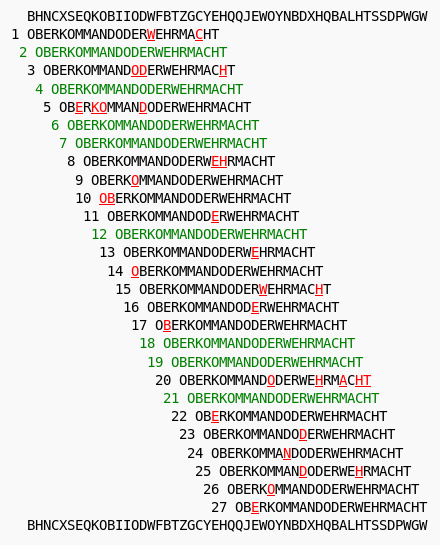
\includegraphics[height=0.8\textheight]{crib}
       \end{center}
      \end{frame}

   \begin{frame}{Enigma}{Verschlüsselung beim deutschen Militär} 
    \begin{block}{Entschlüsselung der Enigma}
     \begin{itemize}[<+->]
      \item 1932: erstes Knacken der Enigma durch den polnischen Mathematiker Marian Rejewski\\
      $\rightsquigarrow$ u.a. Erraten der Walzenverdrahtung
      \item 1938: Erhöhung der Walzenanzahl, Enigma wieder sicher
      \item ab 1939: Kooperation der Polen, Briten und Franzosen zum Knacken der Enigma
      \item ab 1940: kontinuierliche Entschlüsselung der Nachrichten der Luftwaffe und des Heeres
      \item 1943: Entschlüsselung von durchschnittlich mehr als 2500 Funksprüchen pro Tag
     \end{itemize}
    \end{block}
   \end{frame}

   \begin{frame}{Enigma}{Verschlüsselung beim deutschen Militär} 
  
  \textbf{Behebbare Schwächen der Enigma:} \pause
     \vspace{0.5cm}
     
  \begin{block}{}
   \begin{itemize}
    \item nur involutorische, fixpunktfreie Permutationen
    \item unveränderte Verdrahtung der Eintrittswalze
    \item Existenz von Cribbs, Spruchschlüsselverdoppelung
   \end{itemize}
  \end{block}\pause

   \vspace{0.5cm}
   \textbf{Was sind die konezeptionellen Schwächen der Enigma?} \pause
   
   \vspace{0.5cm}
   \begin{alertblock}{}
    \begin{itemize}
	\item Existenz von Codebüchern
	\item öffentliche Übertragung der Grundeinstellung
    \end{itemize}

    \end{alertblock}
  
\end{frame}

\begin{frame}{Public-Key-Kryptography}{Problemstellung, ausgehend von den Schächen der Enigma} 

\begin{itemize}[<+->]
 \item Alice will eine geheime Nachricht an Bob schicken. 
 \item Die beiden haben keine Möglichkeit sich unter vier Augen zu treffen, um einen Geheimschlüssel auszutauschen.
 \item Der Austausch des Geheimschlüssels muss über die öffentliche Kommunikation erfolgen. 
 \item Eine Lauscherin Eve (engl.~eavesdropper) darf anhand der öffentlichen Kommunikation den vereinbarten Geheimschlüssel nur mit einem \underline{zu hohen} Rechenaufwand ermitteln können. 
\end{itemize}
\pause
\vspace{0.5cm}
\begin{exampleblock}{Annahme}
 Eve kann die öffentliche Kommunikation zwischen Alice und Bob zwar abhören, aber nicht beeinflussen.
\end{exampleblock}
 
\end{frame}

\begin{frame}{Public-Key-Kryptography}{Problemstellung, ausgehend von den Schächen der Enigma}

\begin{center}
\begin{tikzpicture}
 \node[pblock] (c1) at (-4, 0) {\nodepart{one} Alice \nodepart{two} Geheimschlüssel};
 \node[pblock] (c2) at (4, 0) {\nodepart{one} Bob \nodepart{two} Geheimschlüssel};
 \node[draw, rectangle, fill=red!20, rounded corners] (ch) at (0, -2) {Eve};
 \draw[-triangle 45] (c1) -- node [above] {öffentlicher Schlüssel} (c2);
 \draw[-triangle 45, decorate, decoration=zigzag] (0, 0) -- (ch);
\end{tikzpicture}
\end{center}
\end{frame}


\begin{frame}{Public-Key-Kryptography}{~} 
 \begin{block}{\underline Public-\underline Key-\underline Cryptography (PKC)}
  Ein einem \tb{Public-Key-Kryptosystem} findet die Vereinbarung der Geheimschlüssels öffentlich statt bzw. ein öffentlicher Schlüssel wird verwendet.
 \end{block}
 \pause
 \vspace{0.5cm}
 \tb{James H.~Ellis}, Mitarbeiter des britischen Geheimdienstes, beschrieb bereits 1970 in einer bis 1997 geheim gehaltenen Arbeit die Idee einer mathematischen \tb{Einwegfunktion} zur Realisierung eines PKC. Er scheiterte jedoch an der konkreten Konzeption eines solchen Kryptosystems.
\end{frame}

\begin{frame}{Public-Key-Kryptography}{Einwegfunktion}
 
 \begin{block}{Einwegfunktion}
  Eine \tb{Einwegfunktion} $f: M \rightarrow N$ ist eine Abbildung mit folgenden Eigenschaften:
  \begin{enumerate}
   \item Es existiert ein Algorithmus, der für jedes $m \in N$ den Bildpunkt $n = f(m)$ in Polynomialzeit berechnet.
   \item Es existiert kein (probabilistischer) Algorithmus, der für einen gegebenen Bildpunkt $n \in f(M)$ einen Urbildpunkt $m \in f^{-1}(\{n\})$ in Polynomialzeit berechnet. 
  \end{enumerate}
  \end{block}
  
  \pause
  \vspace{0.5cm}
  
   \tb{Polynomialzeit:} Anzahl der Schritte des Algorithmus ist beschränkt durch ein Polynom in der Eingabegröße $n$.
   
   \tb{Eingabegröße:} Man denke an die Anzahl der Ziffern $n$ einer Zahl.
   

\end{frame}

\begin{frame}{Public-Key-Kryptography}{Einwegfunktion}
 
\begin{block}{Intuition}
 Man denke an ein Telefonbuch:
 \begin{itemize}
  \item einfach: Finde/Berechne die Telefonnummer von Max Mustermannm im Koblenzer Telefonbuch.
  \item schwierig: Finde/Berechne die Person mit der Telefonnummer 0261-287-2346 im Koblenzer Telefonbuch.
 \end{itemize}
\end{block}

\pause

 \begin{block}{Wunsch}
 \begin{itemize}
  \item Berechnung von Bildpunkten mit polynomiellem Zeitaufwand möglich
  \item Berechnung von Urbildpunkten nur mit exponentiellem Zeitaufwand möglich
 \end{itemize}
\end{block}

\end{frame}

\begin{frame}{Apropos \dots}{~}

\begin{exampleblock}{Die Existenz einer Einwegfunktion würde $P \neq NP$ implizieren:}
Problemstellung: Finde Urbildpunkte unter einer Einwegfunktion.
\vspace{0.5cm}

 Lösungen ($\hat =$ Urbildpunkte unter der Einwegfunktion) können nicht in Polynomialzeit berechnet werden. Das Verifizieren einer Lösung hingegen ($\hat =$ Berechnung des Bildpunktes unter der Einwegfunktion) kann in Polynomialzeit erfolgen.
 \end{exampleblock}
 \pause
 \vspace{0.5cm}
 Das Problem gehört zu den sieben Millenium-Problemen, für deren Lösung das Clay Mathematics Institute in Cambridge im Jahr 2000 ein Preisgeld in Höhe von $1.000.000$\$ ausgelobt hat. 
\end{frame}

\begin{frame}{Public-Key-Kryptography}{Einwegfunktion}
 
 \begin{block}{Kandidaten für Einwegfunktionen}
  \begin{itemize}
   \item \tb{Multiplikation} zweier unterschiedlicher Primzahlen mit \tred{Faktorisierung} als inverser Funktion.
   \item \tb{Potenzieren} von Gruppenelementen mit \tred{Logarithmusbildung} als inverser Funktion.
  \end{itemize}
   \end{block}
  \pause
  
  \vspace{0.5cm}
  
  Man spricht vom 
  \begin{itemize}
   \item \tb{Faktorisierungsproblem großer Zahlen} und
   \item \tb{diskreten Logarithmus-Problem}.
  \end{itemize}

  Bislang sind beide Probleme nur mit \underline{zu hohem} Rechenaufwand lösbar.

\end{frame}


\begin{frame}{Diffie-Hellmann-Schlüsseltausch-Verfahren}{Public-Key-Kryptography}

\begin{exampleblock}{Diffie-Hellman-Schlüsseltausch-Verfahren}
 \begin{enumerate}[<+->]
  \item Alice und Bob einigen sich öffentlich auf eine endliche zyklische Gruppe \tb{$C$} der Ordnung \tb{$q$} und einen Erzeuger \tb{$g$}, \\ d.h. $C = \{g^1, g^2, g^3, \dots\}$ und $|C| = q$.\\
  Beispiel: $p$ eine \glqq große'' Primzahl und $\tb C = \Z_p^* = (\Z_p \setminus \{0\}, \cdot)$
  \item Alice wählt einen zufälligen geheimen Exponenten \tred{$A$} $ < $ \tb{$q$} und berechnet ihren öffentlichen Schlüssel $\tb{a} \coloneqq \tb g^{\tred A} \in \tb C$.\\
  Bob wählt einen zufälligen geheimen Exponenten \tred{$B$} $ < $ \tb{$q$} und berechnet ihren öffentlichen Schlüssel $\tb{b} \coloneqq \tb g^{\tred B} \in \tb C$.\\
  \item Alice und Bob tauschen ihre öffentlichen Schlüssel $\tb a$ und $\tb b$ aus.
  \item Alice und Bob berechnen den gemeinsamen Geheimschlüssel $\tred k \coloneqq \tb b^{\tred A} = \tb a^{\tred B}$. 
 \end{enumerate}
\end{exampleblock}
\pause
\vspace{0.5cm}
Beweis: $\tb b^{\tred A} = (\tb g^{\tred B})^{\tred A} = \tb g^{\tred A \cdot \tred B} = (\tb g^{\tred A})^{\tred B} = \tb a^{\tred B}$
\only<2>{
\vspace{0.5cm}

\begin{block}{Beispiel für $\tb C$}
$p$ eine \glqq große'' Primzahl und $\tb C = \Z_p^* = (\Z/p\Z \setminus \{\overline 0\}, \cdot)$.
 \end{block}}
\end{frame}

\begin{frame}{Diffie-Hellman-Schlüsseltausch-Verfahren}{Public-Key Cryptography}
 \begin{exampleblock}{Diffie-Hellmann Schlüsseltausch-Verfahren}
 Alice und Bob verfügen nun über einen Geheimschlüssel \tred{$k$}. 
 \vspace{0.5cm}
 
 Nun wählen sie ein symmetrisches Kryptosystem und vereinbaren, wie die Schlüssel des Kryptosystems durch die Elemente der Gruppe \tb{$C$} kodiert werden.\\ \pause
  \begin{center}Beides kann öffentlich geschehen!\end{center}
\end{exampleblock}

\end{frame}

\begin{frame}{Diffie-Hellman-Schlüsseltausch-Verfahren}{Public-Key Cryptography}
 Die Sicherheit des Diffie-Hellman-Schlüsseltausch-Verfahrens basiert auf der Annahme, dass zusätzlich zum diskreten Logarithmus-Problem folgende Probleme schwer zu lösen sind:
 \vspace{0.5cm}
 \pause
 \begin{block}{Das Diffie-Hellmann Problem (DH-Problem)}
  Gegeben $\tb g, \tb g^{\tred A}, \tb g^{\tred B} \in C$, berechne $\tb g^{\tred A \cdot \tred B} =: \tred k$.
 \end{block}

\end{frame}

\begin{frame}{Diffie-Hellman-Schlüsseltausch-Verfahren}{Public-Key Cryptography}
 \begin{block}{Vermeiden von Bedienungsfehlern}
  \begin{itemize}
   \item Die Gruppe $\tb C$, deren Erzeuger $g$ und die geheimen Exponenten $\tred A$ und $\tred B$ sind so zu \glqq wählen'', dass Eve aus der Kenntnis von $\tb g$, $\tb a = \tb g^{\tred{A}}$ und $\tb b = \tb g^{\tred{B}}$ die Exponenten $\tred A = \log_{\tb g} \tb a$ und $\tred B = \log_{\tb g} \tb b$ nur mit einem \underline{zu hohen} Rechenaufwand ermitteln kann.
   \item $\tred A$, $\tred B$ und $\tred k$ sind geheim zu halten.
  \end{itemize}
 \end{block}

\end{frame}

\begin{frame}{Diffie-Hellman-Schlüsseltausch-Verfahren}{Public-Key Cryptography}
 \begin{block}{Nachteile}
  \begin{itemize}
   \item Nur der Geheimschlüssel $\tred k$ wird ausgetauscht.
   \item Möchte eine dritte Person Ben eine geheime Nachricht an Alice schicken, so müssen die beiden einen weiteren Geheimschlüssel $\tred {k'}$ vereinbaren, d.h.~Alice als Empfängerin muss wieder aktiv werden.  
  \end{itemize}
 \end{block}
 \pause
 \vspace{0.5cm}
 
  \begin{center} Das Diffie-Hellmann-Verfahren ist daher \tred{ungeeignet} für Einwegkommunikation (z.B.~Emails)! \end{center}  
\end{frame}

\begin{frame}{Public-Key-Kryptography}{Weitere kryptographische Problemstellungen}

\begin{itemize}
 \item Alice möchte geheime Nachrichten empfangen (z.B.~Emails), ohne mit jedem Sender einen separaten Gescheimschlüssel zu vereinbaren.
 \item Alice möchte ihre Nachrichten signieren, so dass jeder Empfänger verifizieren kann, ob Alice die Verfasserin ist. (Authentizität/Digitale Signaturen)
 \item Bob möchte sicher gehen, dass die Nachricht, die er von Alice erhalten hat, nicht nachträglich verändert wurde. (Integrität)
\end{itemize}
\end{frame}

\begin{frame}{Der Faktor Mensch}{Eine Schlussbemerkung zur Sicherheit moderner Kryptosysteme}
\begin{alertblock}{~}
 Die sogenannten \tb{Seitenkanalattacken} bedingt durch
 \begin{itemize}
  \item \textbf{Implementationsfehler} und
  \item \textbf{Bedienungsfehler} 
 \end{itemize}
 sind die größten Sicherheitslücken moderner Kryptosysteme.
\end{alertblock}

\end{frame}

\begin{frame}{Kurzüberblick über die Vorlesung}{Kryptographie}

\begin{enumerate}[<+->]
 \item  \tb{Gibt es sichere Kryptosysteme?} \\
 Perfekte Geheimhaltung
 \item \tb{Wie funktioniert WLAN-Verschlüsselung?}\\
 Blockchiffren, AES und Pseudozufallszahlen 
 \item \tb{Wie funktioniert geheime Kommunikation via Email ohne vorheriges Vereinbaren eines gemeinsamen Geheimschlüssels?}\\
 Public-Key-Kryptosysteme (RSA, Rabin, ElGamal), Einwegfunktionen, Primzahltests
 \item \tb{Wie kann Google überprüfen, dass ich mich einlogge, ohne dass Google mein Passwort kennt?}\\
 Identifikation
 \item \tb{Wie kann ein vergessenes Passwort rekonstruiert werden, ohne es bei einer einzelnen Person zu hinterlegen?} \\
 Secret Sharing
\end{enumerate}
 
\end{frame}


\end{document}


